% Modelo de slides para projetos de disciplinas do Abel
\documentclass[aspectratio=169,11pt]{beamer}

\usetheme[%
 sectionpage=none,%
 subsectionpage=progressbar%
 ]{metropolis}

\usepackage[czech]{babel}
\usepackage{graphicx}
\usepackage{enumitem}
\usepackage{amsmath}
\usepackage{mathtools}
\usepackage{tcolorbox}

\tcbset{%
 sharp corners=all,%
 boxsep=7pt,%
 fonttitle=\bfseries,%
 colback=gray!30!white,%
 colframe=mDarkTeal,%
 boxrule=1pt%
}

\title{ALGORITMUS}
\date{\today}
\author{Adam Klepáč}
\institute[GEVO]{Gymnázium Evolution Jižní Město}

% enumerate global settings
\setlist[enumerate,1]{label=\arabic*.}
\setlist[enumerate,2]{label=\alph*)}

\begin{document}

\begin{frame}
 \begin{columns}
  \begin{column}{.45\textwidth}
   \maketitle
  \end{column}
  \begin{column}{.45\textwidth}
   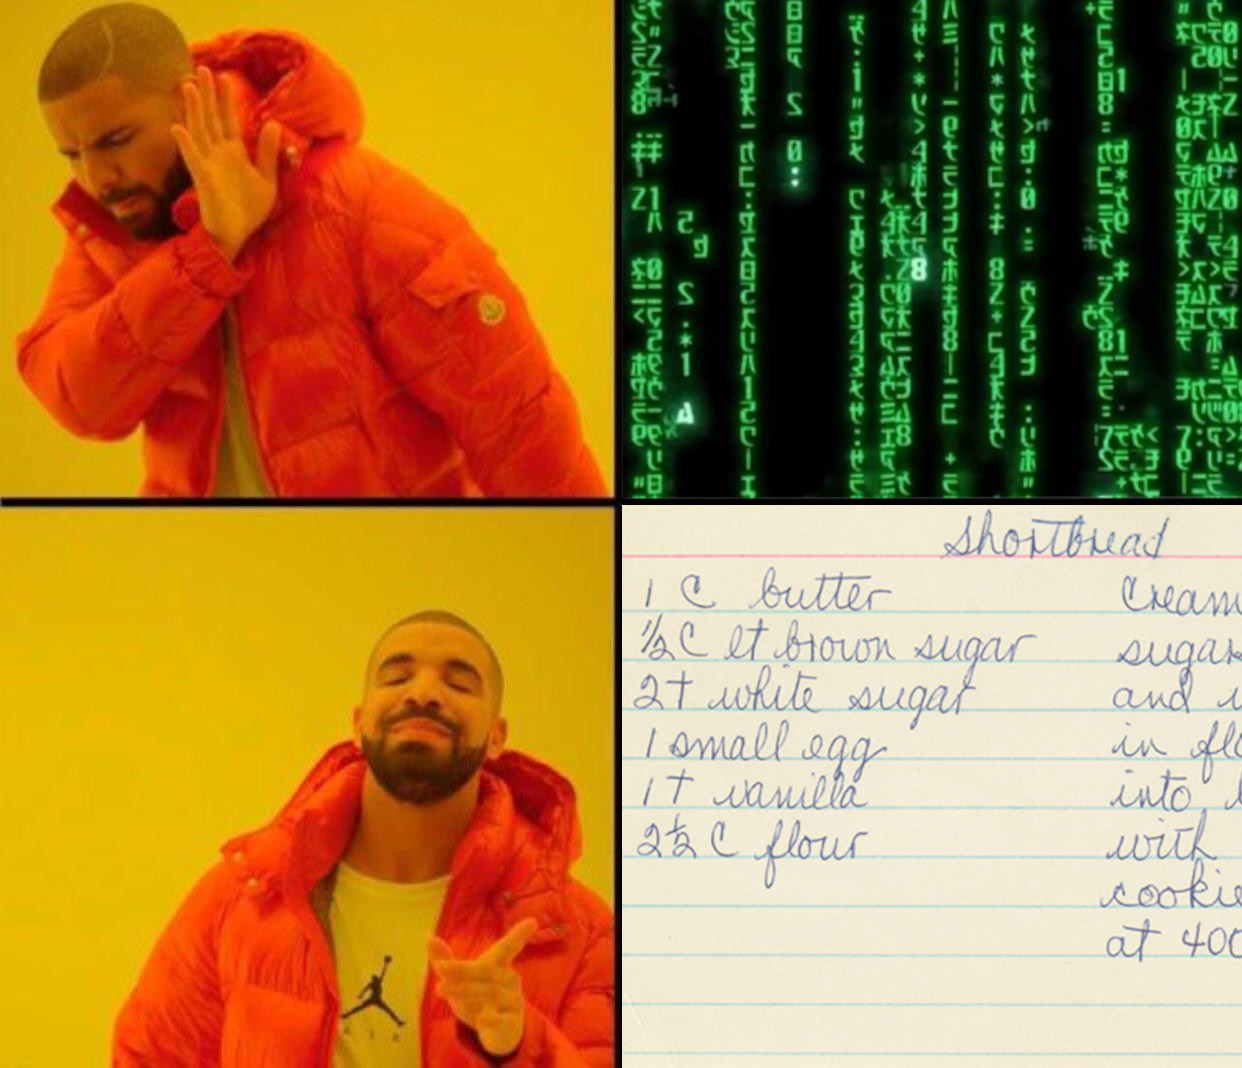
\includegraphics[width=\textwidth]{intro-meme}
  \end{column}
 \end{columns}
\end{frame}

\begin{frame}
 \frametitle{Obsah}
 \tableofcontents
\end{frame}

\section[Co je algoritmus?]{Co je algoritmus?}

\subsection[Příklady]{Příklady}

\begin{frame}
 \frametitle{Recept na mramorovou bábovku}
 \begin{block}{Postup}
  \begin{enumerate}
   \item Smíchejte cukr s vejci, přidejte olej, mouku, mléko, prášek do pečiva,
    vanilkový cukr a dobře promíchejte.
   \item Rozdělte těsto do dvou misek. Do jedné misky přidejte podle chuti
    nastrouhanou kůru z citronu.
   \item Do další misky s těstem dejte holandské kakao také podle chuti.
   \item Nalijte do vymazané formy a pečte na 200 °C 45–50 min.
   \item Po upečení ještě horkou vyklopte na talíř. Krájejte vlažnou.
  \end{enumerate}
 \end{block}
\end{frame}

\begin{frame}
 \frametitle{Jak si zavázat tkaničky}
 \begin{block}{Postup}
  \begin{enumerate}
   \item Udělejte uzel.
   \item Udělejte mašličku na pravé tkaničce.
   \item Levou tkaničkou mašličku omotejte.
   \item Pravým ukazováčkem prostrčte pravou mašličku očkem směrem za pravým
    palcem.
   \item Chytněte vrcholy mašliček.
   \item Utáhněte.
  \end{enumerate}
 \end{block}
\end{frame}

\begin{frame}
 \frametitle{Sčítání pod sebou}
 \begin{block}{Postup}<1->
  \begin{enumerate}
   \item<2->\label{item:sum-1} Sečtěte číslice na poslední pozici obou čísel.
   \item<3-> K součtu přičtěte přebytek.
   \item<4-> Výsledný součet napište.
   \item<5-> 
    \begin{enumerate}
     \item Je-li součet větší než 10, nastavte přebytek na 1.
     \item Je-li součet menší než 10, nastavte přebytek na 0.
    \end{enumerate}
   \item<6-> Zapomeňte/smažte poslední číslice obou čísel.
   \item<7-> Pokud ještě oběma číslům zbývají nějaké číslice, opakujte krok
    \ref{item:sum-1}
  \end{enumerate}
 \end{block}
\end{frame}

\subsection[Protipříklady]{Protipříklady}

\begin{frame}
 \frametitle{Já věřím, že poletím!}
 \begin{block}{Postup}
  \begin{enumerate}
   \item Vystoupejte na nejvyšší vrchol v okolí 5 km.
   \item Vzneste se.
   \item Udělejte si selfie.
   \item Uploadněte je na Instagram.
   \item Leťte 10 km na západ rychlostí zvuku ve vodě.
   \item Přistaňte.
   \item Zkontrolujte liky a commenty.
  \end{enumerate}
 \end{block}
\end{frame}

\begin{frame}
 \frametitle{Nerozhodná navigace}
 \begin{block}{Postup}
  \begin{enumerate}
   \item Jsme připraveni. Řiďte bezpečně.
   \item Pokračujte rovně deset minut až po odbočku Turnov/Liberec/Mnichovo
    Hradiště.
   \item Sjeďte vpravo.
   \item Z kruhového objezdu vyjeďte kterýmkoli výjezdem.
   \item Pokračujte rovně pět minut.
   \item Cíl.
  \end{enumerate}
 \end{block}
\end{frame}

\begin{frame}
 \frametitle{Největší společný násobek}
 \begin{block}{Postup}
  \begin{enumerate}
   \item Máte dána přirozená čísla $A$ a $B$.
   \item Položte $N \coloneqq AB$.
   \item Dokud $A$ dělí $N$ a $B$ dělí $N$, opakujte následující kroky:
    \begin{enumerate}[label=\roman*.]
     \item Položte $N \coloneqq NA$.
     \item Položte $N \coloneqq NB$.
    \end{enumerate}
   \item Vypište $N$.
  \end{enumerate}
 \end{block}
\end{frame}

\subsection[Neformální popis]{Neformální popis}

\begin{frame}
 \frametitle{Popis pomocí vlastností}
 Algoritmem nazveme \alert{chronologickou sadu příkazů} splňující
 následující tři vlastnosti.
 \pause
 \begin{tcolorbox}[title=Vlastnost 1: splnitelnost,width=.8\textwidth,center]
  Příkazy musejí být splnitelné \alert{z pohledu plnitele}.
 \end{tcolorbox}
\end{frame}

\begin{frame}
 \frametitle{Popis pomocí vlastností}
 Algoritmem nazveme \alert{chronologickou sadu příkazů} splňující
 následující tři vlastnosti.
 \begin{tcolorbox}[title=Vlastnost 2: jednoznačnost,width=.8\textwidth,center]
  Příkazy musejí být jednoznačné \alert{z pohledu plnitele}.
 \end{tcolorbox}
\end{frame}

\begin{frame}
 \frametitle{Popis pomocí vlastností}
 Algoritmem nazveme \alert{chronologickou sadu příkazů} splňující
 následující tři vlastnosti.
 \begin{tcolorbox}[title=Vlastnost 3: konečnost,width=.8\textwidth,center]
  Příkazy musejí vyžadovat jen konečně mnoho prostoru a času.
 \end{tcolorbox}
\end{frame}

\begin{frame}
 \centering\Huge Díky za pozornost.
\end{frame}

\end{document}
